In the different tests in which we have used PMT, we were interested in two different main objectives. On the one hand, we were interested in knowing the amount of incident photons that reached the PMT photocathode, which can be interesting, for example, to characterize fibers, and, on the other hand, we were interested in the energy of each event that occurred, which can be interesting, for instance, to obtain an energy spectrum or to discriminate events based on their energy (for knowing the origin of these events and counting only interesting events).

In the first case, if we want to know how many photons have reached the photocathode, we have to work without the internal gain of the PMT. The reason for this is that it introduces a large uncertainty in the measurement. The use of this internal gain could be interesting in other situations such as when we need to know the energy of the event because, as we saw in the section \ref{subsubsec:PMTs}, its use greatly enlarges our signal, a factor of the order of $10^6$, and, due to that, it is easier to process and analyze it.

For working without the internal gain of the PMT we need to avoid the use of the electron multiplication stage that we saw in section \ref{subsubsec:PMTs}. To achieve this, we design, build and test special PCBs, whose electronic scheme is shown in figure \ref{}, in which we short-circuit all the dindes and read the signal directly from the photocathode.

PHOTO AND ELECTRONIC DESIGN.

This PCB is designed to be powered with positive supply voltage which is less thant the normal situation $[0-400~\volt]$. The reason of this lower supply voltage is that we don't need to create a voltage difference between each pair of dynodes in the chain (we only need to create a voltage difference between the photocathode and the first dinode).

In this case, the output signal of our photosensor is very fast and small (currents of the order of tens of nanoamperes\footnote{$1~\ampere=10^{9}~\nano\ampere$}) and we need a special system to analyze these types of currents. The system which we have chosen is Keithley 6487 Picoammeter/Voltage Source \cite{DataSheetKeithley6487}, which is a commercial system from the Keithley company, because it has some interesting options for this study such as automatic baseline correction, the ability to read signals as small as picoamps and the ability to perform some interesting mathematical operation, such as the average of N measurements with the associated statistical error, where N is programmable by the user ($N=100$ in all our studies).

With this configuration we can measure the output current of our photosensors and, from it, quantify how many photons have been detected by the PMT photocathode using the equation \ref{eq:NumPhotonsFromIntensityPMT}:

\begin{equation}
Nº\gamma/\sec = \frac{\left( I_{PMT} - I_{DC} \right)}{q_e \cdot{} QE \cdot{} CE}
\label{eq:NumPhotonsFromIntensityPMT}
\end{equation}

Where $I_{PMT}$ is the output current of the PMT when it detects photons and $I_{DC}$ is the dark current of the PMT. This equation takes into account the quantum efficiency, which is close to $30\%$ for the PMTs used, and the capture efficiency in the dyndes, which is equal to 1 because we read the signal directly from the photocathode. In addition, it is taken into account that, due to the photoelectric effect in which this detection consists, each detected photon only generates one electron, whose charge is $q_e$.

In the second case, if we want to know the energy of the event that occurred, we need to work with the internal gain of the PMT. For that we will use the electron multiplication stage that we saw in section \ref{subsubsec:PMTs}.

In all our studies we have used several PMTs in our experiments (two or four depend on the case). The electronic schematics used, which are shown in figure \ref{subfig:ElectronicConfiguraiton2PMT} and \ref{subfig:ElectronicConfiguraiton2PMT} respectively, are based on various NIM technology modules\footnote{The Nuclear Instrumentation Module (NIM) is a standard specification convention for electrical and mechanical parameters defined in electronic modules used in experimental nuclear and particle physics.}.

\begin{figure}[htbp]
 \centering
  \subfloat[Electronical configuraiton scheme used to measure with two PMTs.]{
   \label{subfig:ElectronicConfiguraiton2PMT}
    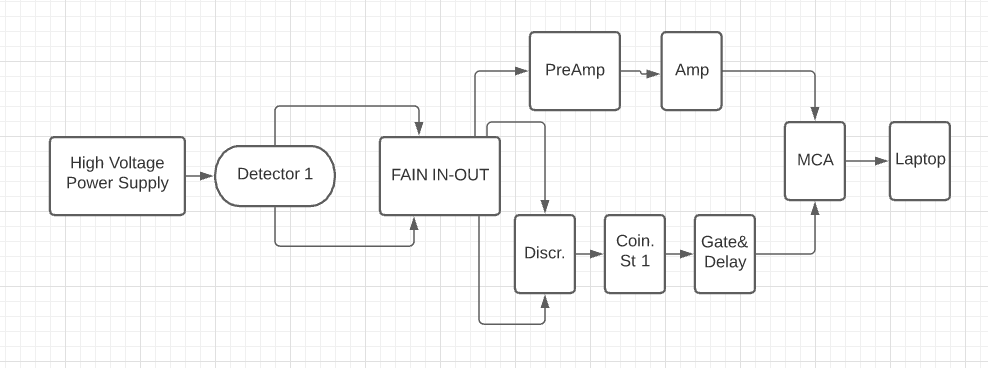
\includegraphics[width=1.0\textwidth]{3DesignPrinciples/32Tritium_detector/Electronical_Scheme_1_detector.png}}
    \newline
  \subfloat[Electronical configuraiton scheme used to measure with four PMTs.]{
   \label{subfig:ElectronicConfiguraiton4PMT}
    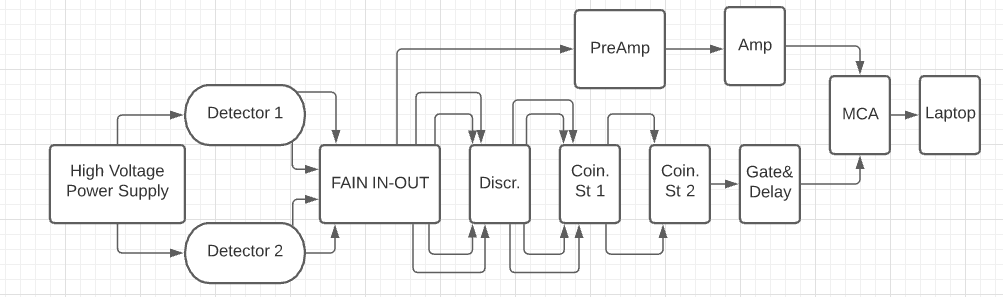
\includegraphics[width=1.0\textwidth]{3DesignPrinciples/32Tritium_detector/Electronical_Scheme_2_detectors.png}}
 \caption{Schemes of different electronic configuration used to measure with PMT.}
 \label{fig:ElectronicConfiguraitonsPMT}
\end{figure}

The PMTs used in each situation are feeded with the voltage supply "TC 952 High Voltage Supply" from Tennelec \cite{DataSheetHVSupplyTennelec}. It has four channels for feeding up to four different PMTs so it is enough for both configurations. In some situations we need to work with both configurations at the same time, that's, with six PMTs at the same time.  In this cases other voltage supply had been used, called  "HV Power Supply N 1130-4" from "Wenzel Elektronik" \cite{DataSheetHVSupplyWenzel} company with which we get 4 additional channels for feeding PMTs. The high voltage used in each case will be named in each specific situation.

As you can see in the figures \ref{subfig:ElectronicConfiguraiton2PMT} and \ref{subfig:ElectronicConfiguraiton2PMT}, in both electronic configurations there are two different paths that must be followed by the output signals of each PMT, the amplification part and the time coincidence part. Therefore, the first module we need is the analogic FAN IN-OUT module which is used to duplicate the input signal.

The module used is the "Quad linear FAN IN-OUT MODEL 740" module from the company "Philips Scintific" \cite{DataSheetFANINOUT}. With this module we can obtain up to 4 output signals (we only need two) that are totally identical to each input signal. For each PMT we have two identical output signals. One will be used as the input for the amplification part and the other will be used as the input for the time coincidence part.

\begin{itemize}

\item{} The amplification part, which is the same for both electronic configurations, figures \ref{subfig:ElectronicConfiguraiton2PMT} and \ref{subfig:ElectronicConfiguraiton4PMT}, is used to process and amplify the output signal and it is the same for both configurations. We have to take into accout that we have only used the signal from one PMT for the amplification part. We could have added a stage where we add the four PMT output signals and it would probably improve our results, but since our ultimate goal is to work with SiPM, we have not delved into that.

The electronic path we have followed to achieve this amplification is:

\begin{enumerate}

\item{} In this part we introduce one of the output signals of the previous module (FAN IN-OUT) in a preamplifier that is used to prepare the signal to be amplified, appendix \ref{App:ElectronicModulesNIM}. The preamplifier used is "MODEL 9326 FAST PREAMP" from ORTEC \cite{DataSheetPreAmp}.

\item{} The output signal from the preamplifier is introduced into the amplifier where it will be converted to a positive signal with a shape close to the Gaussian function and an amplification factor will be applied. The amplifier modules used on this studies are "model 575A" and "model 671", both from ORTEC company \cite{DataSheet575Amp}, \cite{DataSheet671Amp}. The output signal for 575A module is shown in figure \ref{fig:InputSignalsMCA}, green color.

\end{enumerate}

\item{} The time coincidence part is used to obtain the coincidence gate that will be used to indicate when we have to save the amplified signal (which is when all the PMT output signals are in time coincidence). Only the saved output signal will be used for the analysis. 

This part is practically the same in both cases with just one additional step when we use four PMTs. The electronic path followed in the time coincidence part is:

\begin{enumerate}

\item{} The second output signals of the FAN IN-OUT module for each PMT are introduced into a discriminator module where we obtain an output logic signal with height of $-1.2~\volt$ and width of $240~\nano\second$ when a threshold, the one programmed by the user, is exceeded. The discriminators used in our experiments are  "Octuple Constant-Fraction Discriminator CF8000" module from ORTEC company \cite{DataSheetDiscriminator} and "4 channels discriminator model 84" from CAEN company. These four output signals are shown in figure \ref{subfig:signalInAllPMTsBothDetector} for four PMTs in coincidence.

\item{} Now is the time to make time coincidences. As we will see in the section \ref{subsec:SetUpActiveShield} and chapter \ref{chap:Prototypes}, we have two photosensors in each detector, so we will do time coincidences in pairs of photosensors, PMTs in this case.

Therefore, each pair of output logic signals of the discriminator module (attached to two PMTs that are in the same detector) will reach a different channel of the coincidence module and generate an output signal, with a height of $-1.4~\volt$ and width of $20~\ns$, when a time coincidence has occurred on them.

This first time coincidence stage is used to remove the detection of  external light or dark current of PMTs from  in the saved measurements. This is because this module only generate logic output signals when both PMTs have detected photons at the same time, indicating that these photons are coming from the coupled scintillator.

The time coincidence modules used are "Coincidence Unit Model 465" from LeCroy \cite{DataSheetCoincidenceLeCroy} and "Coincidence Type N6234" from CERN-NP \cite{DataSheetCoincidenceCERN}.

\item{} The next step, which is included only when working with four different PMTs, is used to do time coincidence between two different detectors. It could be interesting, for exapmle, to detect hard cosmic radiation as we will be in the \ref{subsec:SetUpActiveShield} section.

If we want to do time coincidences between both detectors, we have to use the logical output signals of the previous step (output of the coincidence module) as input of another coincidence stage similar to the previous one. In this case, which is only used when we have four PMTs, we will have a logical output signal with the same parameters, height of $-1.4~\volt$ and width of $20~\nano\second$ when both detectors have detected events at the same time. The modules used is the same named in the previous point.

In the figure \ref{fig:DifferentCoincidences} we have shown all the different situations that we can have with the previous two steps. There we have four logical signals from four PMTs. The two first signals (channel one and two) come from two PMTs connected to one detector and the other two signals (channels three and four) come from PMTs connected to another detector.

\begin{enumerate}
\item{} In figure \ref{subfig:signalInOnePMT} we can see that only one PMT (channel two) has detected an event. As the second PMT connected to the same detector (channel one) did not detect this event, it indicates that the detected photons did not come from the scintillator. In this case, the time windows (output from coincidence module, stage 1) will not be opened and this event will not be saved.

\item{} In figures \ref{subfig:signalInTwoPMTOneDetector} and \ref{subfig:signalInTwoPMTOtherDetector} we can see that two PMT signals connected to the same detector have detected an event but the others have not. It means that it is an event that has only been detected by one detector. If we are using the second stage of time coincidence, the time window will not open to save this event.

\item{} In figure \ref{subfig:signalInAllPMTsBothDetector} we can see that, in this case, all signals have detected the event. It means that it is an event that has been detected for both detectors. In this case, a time window will be created to save this event.

\begin{figure}[htbp]
 \centering
  \subfloat[Event detected in only one PMT.]{
   \label{subfig:signalInOnePMT}
    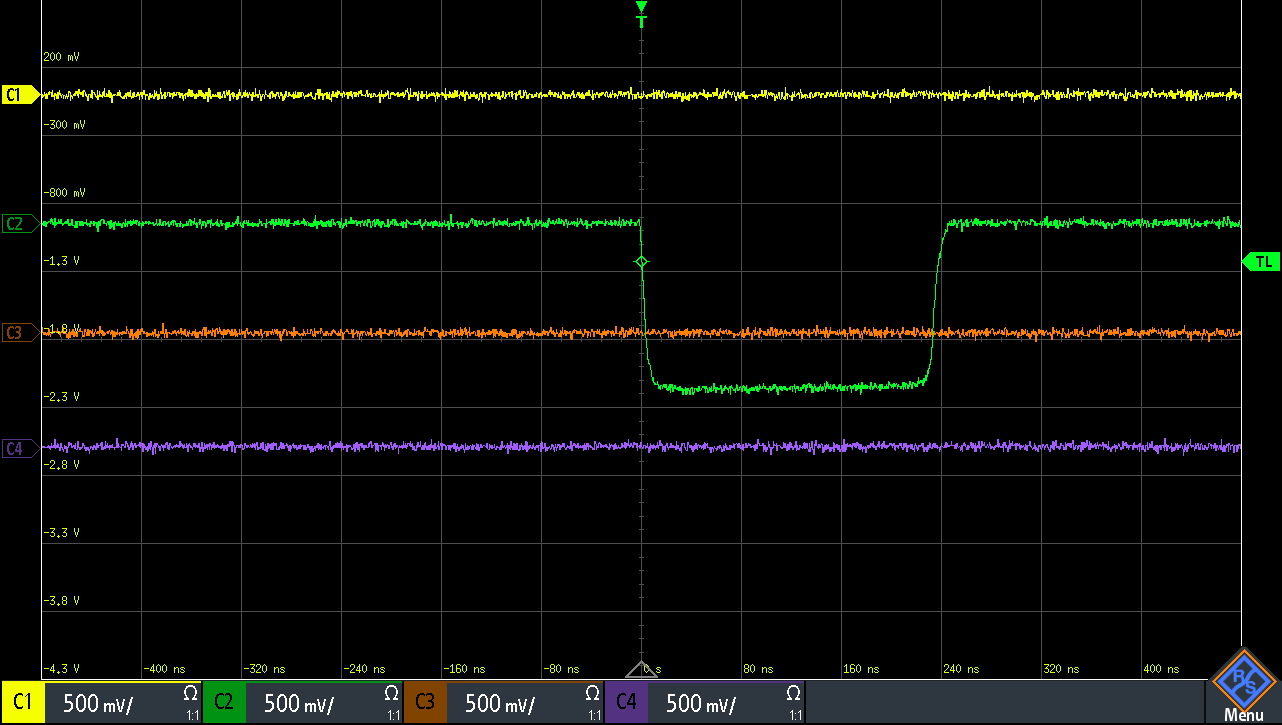
\includegraphics[width=0.5\textwidth]{3DesignPrinciples/32Tritium_detector/1_coincidences.png}}
  \subfloat[Event detected in two PMTs, one detector.]{
   \label{subfig:signalInTwoPMTOneDetector}
    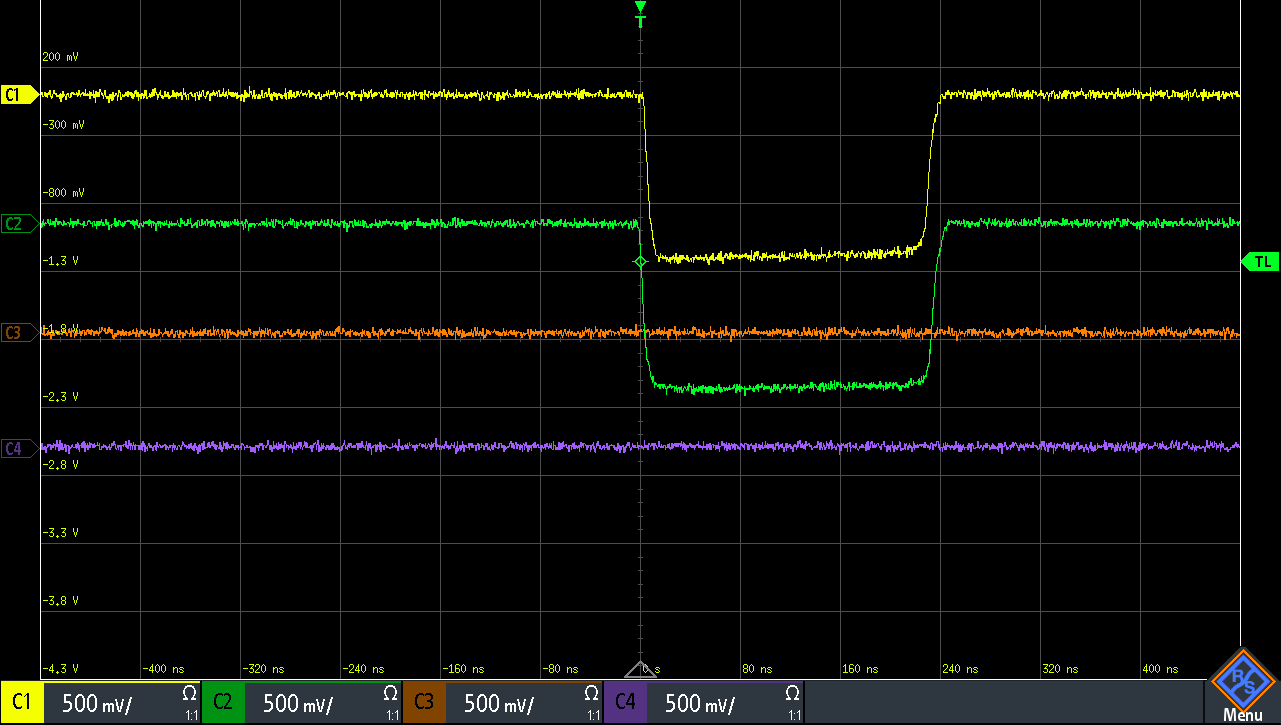
\includegraphics[width=0.5\textwidth]{3DesignPrinciples/32Tritium_detector/2_coincidences_1.png}}
   \newline
  \subfloat[Event detected in two PMTs, other detector.]{
   \label{subfig:signalInTwoPMTOtherDetector}
    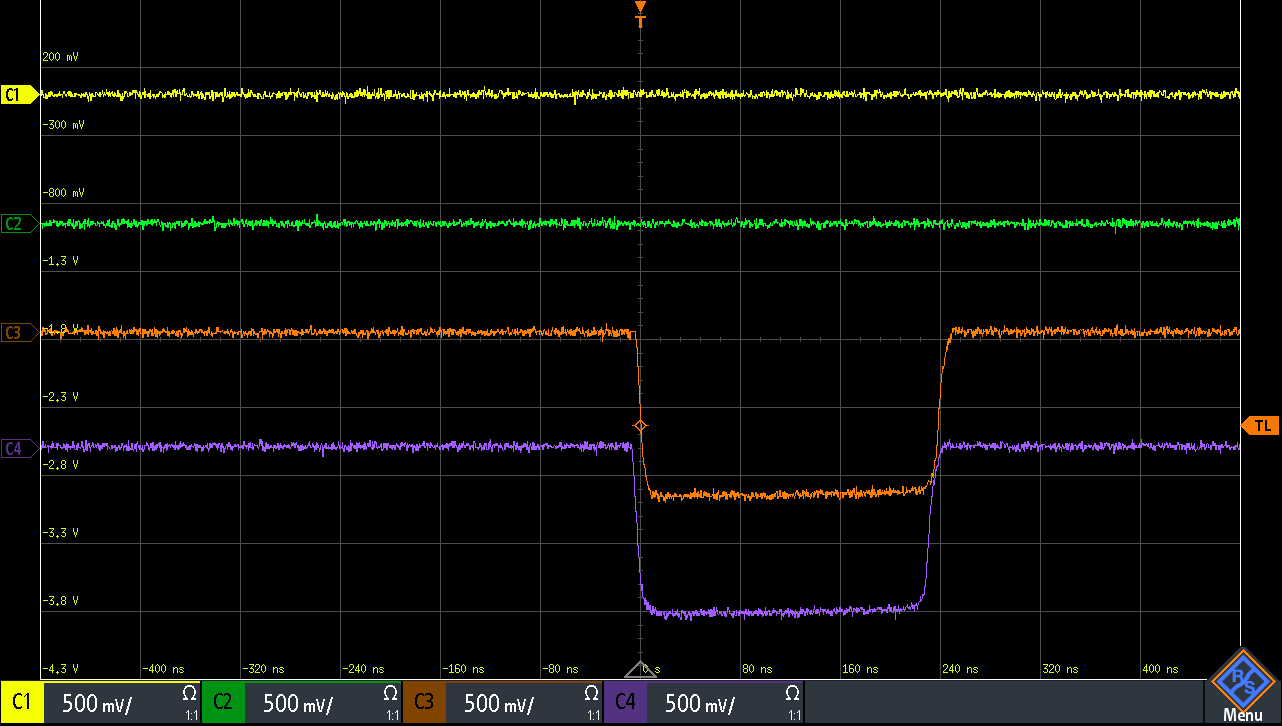
\includegraphics[width=0.5\textwidth]{3DesignPrinciples/32Tritium_detector/2_coincidences_2.png}}
    \subfloat[Event detected in all PMTs, both detector.]{
   \label{subfig:signalInAllPMTsBothDetector}
    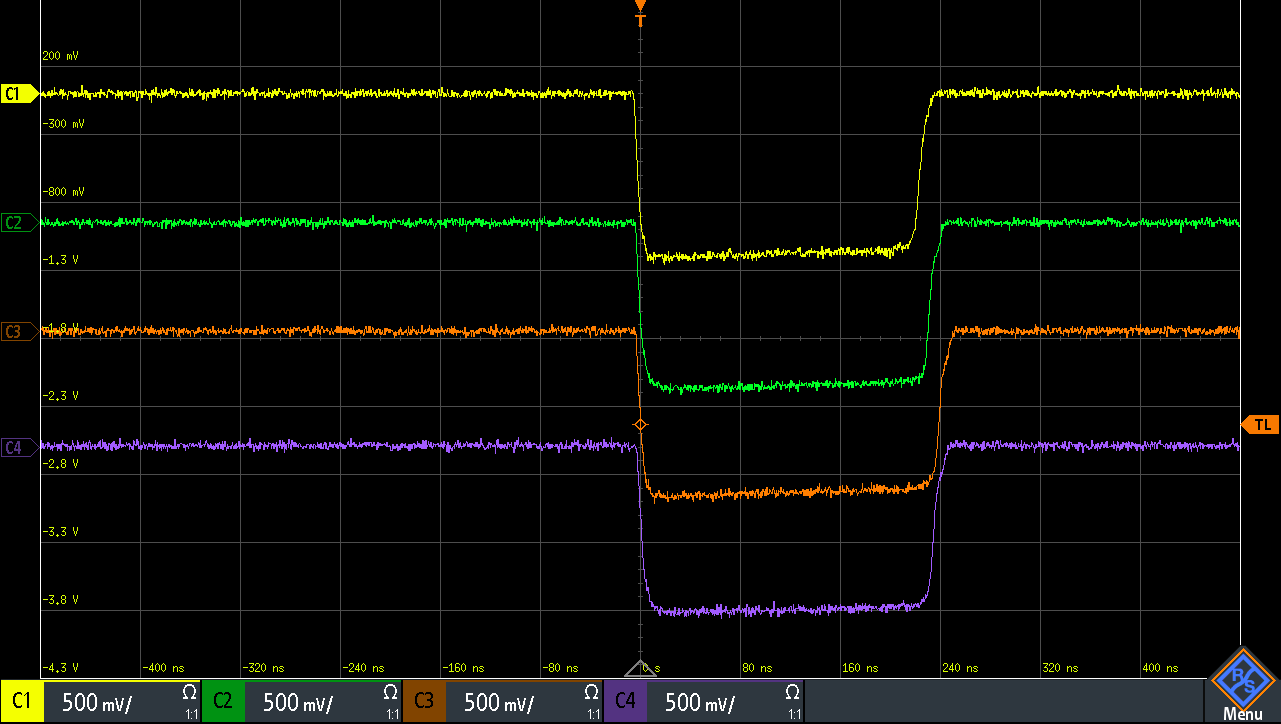
\includegraphics[width=0.5\textwidth]{3DesignPrinciples/32Tritium_detector/4_coincidences.png}}
 \caption{Different situation that can happen when we do time coincidences with PMTs.}
 \label{fig:DifferentCoincidences}
\end{figure}


\end{enumerate}

\item{} Finally, the logical output signal of the coincidence module used, which indicates that all the PMTs used in our study are in temporal coincidence, is introduced in the "Gate and Delay Generator, model 416A" of the company ORTEC \cite{DataSheetGateAndDelay}. With this NIM module we obtain a positive logical signal, shown in the figure \ref{fig:InputSignalsMCA}, orange color, with a height of $8~\volt$ and width of $2~\mu\second$.

\end{enumerate}

\end{itemize}

At the end, we have two different signals, shown in figure \ref{fig:InputSignalsMCA}, which will be introduced in the MCA 8000D, Pocket MCA from AMPTEK company \cite{DataSheetMCA} to be saved. On the one hand we have an analog signal (output from the amplifier module) that has information about the event that has been detected (its energy, detection time, etc.) and this is the signal whose information we will save for analyzing. On the other hand we have a logic signal (output from the Gate and Delay Generator module) that indicates when we have to save the amplified signal, that is, when all our PMTs used in our experiment have detected an event at the same time.

\begin{figure}[htbp]
\centering
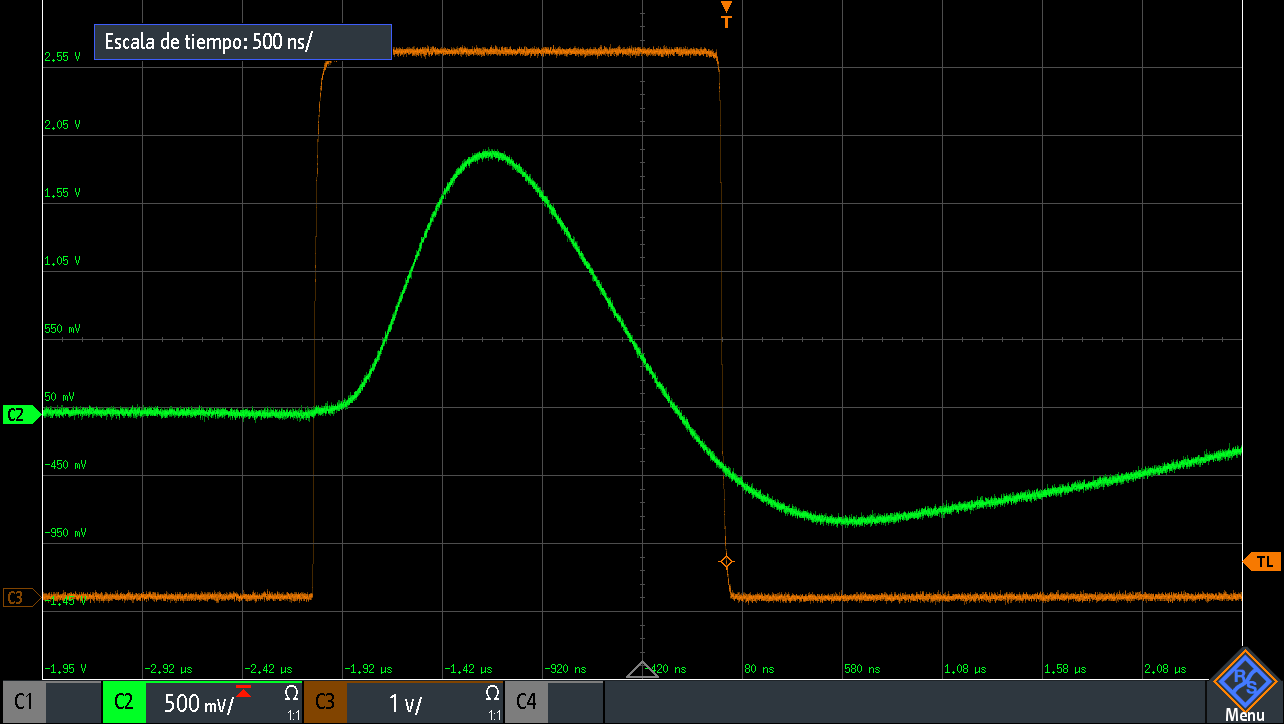
\includegraphics[scale=0.3]{3DesignPrinciples/32Tritium_detector/Input_MCA.png}
\caption{Signal amplificated and logical gate (input signals of MCA).\label{fig:InputSignalsMCA}}
\end{figure}


The information that will be saved and histogramed in the MCA is the weight of the signal, which is proportional to the energy of the detected event, explained in the appendix \ref{App:ElectronicModulesNIM}. An example of histogram as output of the MCA is shown in figure \ref{fig:EnergySpectrum4PMTs}.

\begin{figure}[htbp]
\centering
%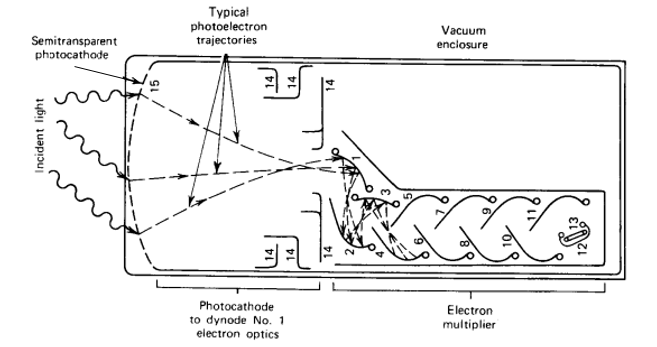
\includegraphics[scale=0.6]{3DesignPrinciples/32Tritium_detector/PMTschematic.png}
\caption{Energy spectrum obtained with the electronic configuration explained in this section for four PMTs.\label{fig:EnergySpectrum4PMTs}}
\end{figure}
